\documentclass[../PHYS306Notes.tex]{subfiles}

\begin{document}
\subsection{Worksheet - Review of Noninertial Frames}

\begin{center}
    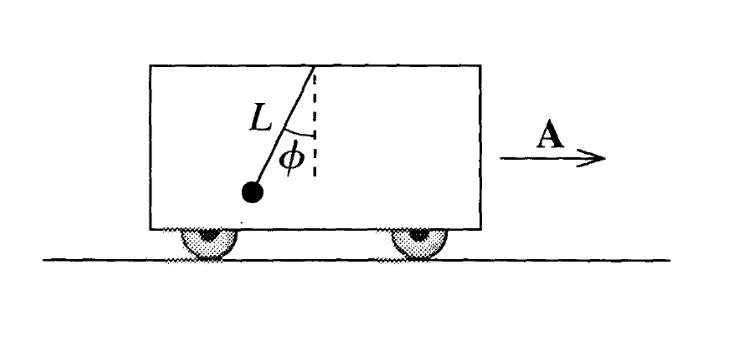
\includegraphics[scale=0.5]{Lecture-14/w14-img1.png}
\end{center}

\begin{p}
A pendulum is inside of a railcar that is accelerating in the x-direction with acceleration $A$  Find the equilibrium value of the angle $\phi$. 
\end{p}
\begin{s}
Apply Newton's law in the non-inertial frame:
\[m\ddot{\v{r}} = \v{F} - m\v{A}\]
We have that the forces in the inertial frame are given by $\v{F} = m\v{g} + \v{T}$, (gravity and tension) so:
\[m\ddot{\v{r}} = m\v{g} + \v{T} - m\v{A}\]
Grouping terms:
\[m\ddot{\v{r}} = \v{T} + m(\v{g} - \v{A})\]
Where we may call $\v{g} - \v{A}$ the effective acceleration, $\v{g}_{eff}$. By trigonometry, the equilibrium angle would be given by:
\[\tan\phi_{eq} = \frac{A}{g}\] As can be seen from the diagram below:
\begin{center}
    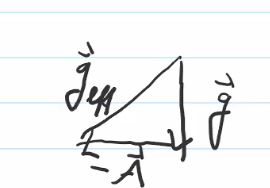
\includegraphics[scale=0.8]{Lecture-14/w14-img2.png}
\end{center}
\end{s}

\begin{center}
    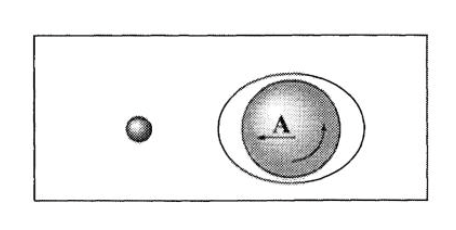
\includegraphics[scale=0.75]{Lecture-14/w14-img3.png}
\end{center}
\begin{center}
    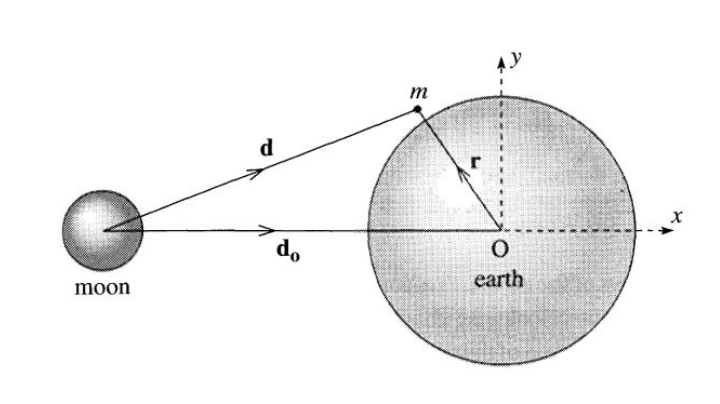
\includegraphics[scale=0.75]{Lecture-14/w14-img4.png}
\end{center}
\begin{p}
The earth and moon orbit each other, while both earth and moon frames of reference are accelerating. Find the acceleration in each frame of reference. 
\end{p}
\begin{s}
In the inertial frame, the forces on the test mass on the surface of the Earth is given by:
\[\v{F} = m\v{g} - gM_{m}m\frac{\hat{\v{d}}}{d^2}\]
Where $M_m$ is the mass of the moon. The Earth is not an inertial system, so it experiences some acceleartion. The acceleration of the center of the mass of the earth is given by:
\[\v{A} = -GM_{m}\frac{\hat{\v{d}}_0}{d^2_0}\]
Hence we have:
\[m\ddot{\v{r}} = m\v{g} - GM_mm\left(\frac{\hat{\v{d}}}{d^2} - \frac{\hat{\v{d}}_0}{d^2_0}\right) = m\v{g} - \v{F}_{tidal}\]
The tidal force is the vector difference between if the mass is at the surface of earth vs. at the center of mass of the earth. This results in tidal effects at either side of the earth, with the same magnitude and in the opposite direction ($\hat{\v{d}}$ and $\hat{\v{d}}_0$ are parallel at these two points, so the effect is maximal). We end up with a bulge on both sides of the Earth. At the top and bottom, we have that the x components cancel by symmetry, so we only have the y component (weaker effect, inwards pointing). This is shown in the diagram below:
\begin{center}
    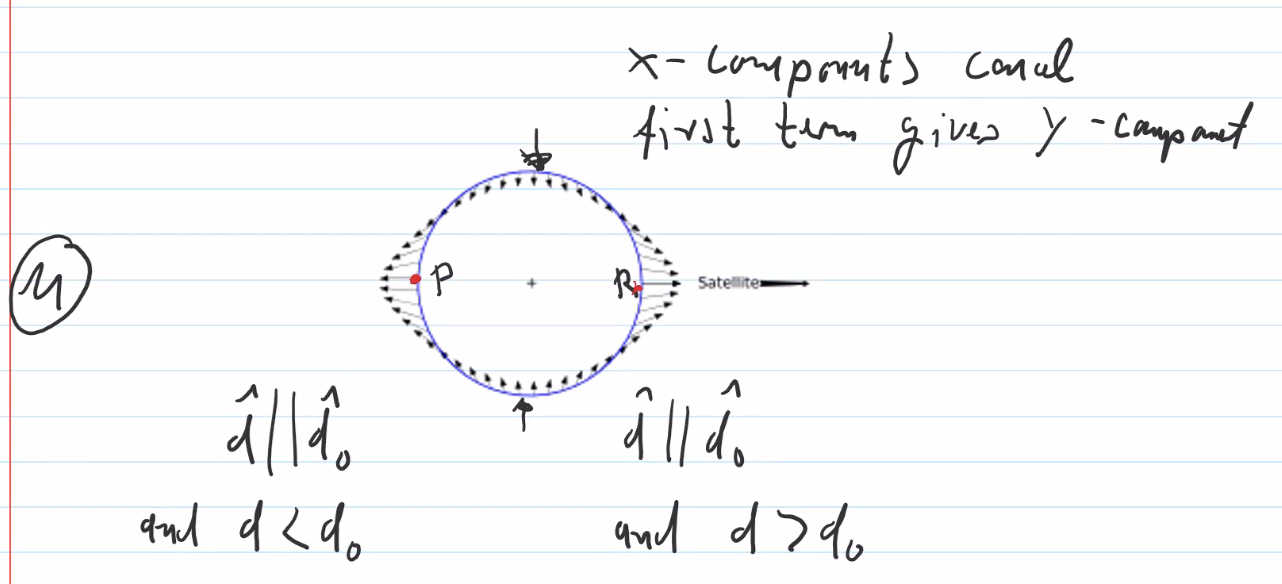
\includegraphics[scale=0.5]{Lecture-14/w14-img5.png}
\end{center}
\end{s}

\begin{p}
Find the equation of motion for a particle on the surface of the ocean of the earth, in the earth’s frame of reference. 
\end{p}
\begin{s}

\end{s}
\end{document}